\documentclass[final]{beamer} % beamer 3.10: do NOT use option hyperref={pdfpagelabels=false}!

%\documentclass[final,hyperref={pdfpagelabels=false}]{beamer} % beamer 3.07: get rid of beamer warnings

\mode<presentation>{\usetheme{dsmanchester}}

% Portrait, A0 poster. Set scale as desired, but 1.o3 gives easily readable text when printed.
\usepackage[orientation=portrait, size=a0, scale=1.3]{beamerposter}
\usepackage{booktabs}
\usepackage{caption}
\usepackage{subcaption}
\usepackage{adjustbox}
% Set height of page for use in arranging text boxes, after accounting for
% heading, footer etc. This is a bit of a hack, ideally latex should figure
% this out for itself!

\newcommand{\rpm}{\raisebox{.2ex}{$\scriptstyle\rpm$}}

\newlength{\columnheight}
\setlength{\columnheight}{1025mm}
\setlength{\tabcolsep}{12pt}

                  
% Define the header information
\title{Unsupervised Task Discovery for \\ Multi-Task Acoustic Modeling}
\author{\large{\textit{Josh Meyer}}}
\institute{\texttt{joshua.richard.meyer@gmail.com  |  @\_josh\_meyer\_  |  jrmeyer.github.io}}


% Put any other packages or custom macros in here:



% Now start the actual poster
\begin{document}

% Header is automatically generated from the command defined in the theme
% file, the information above and the logos in the logo folder.


% Start of the body:
\begin{frame}
  \begin{columns}
    %% Leftmost column:
    \begin{column}{0.3\textwidth}
      % For some reason we need parbox to get it to arrange the boxes
      % with evenly spaced gaps
      \parbox[t][\columnheight]{.9\textwidth}{

        \vspace{1cm}
        
        \begin{block}{Abstract}
          \begin{itshape}   % italic abstract
            \begin{itemize}
            \item Multi-Task Learning works (good for low-resource languages)
            \item However, tasks are hard to make
            \item Better to discover tasks automatically
            \item Experiment with k-means on MFCCs
            \item Data == 1.5 hours of Kyrgyz audio-book
            \item Initial Results Promising
            \end{itemize}
          \end{itshape}
        \end{block}

        \vfill
        
        \begin{figure}[!htbp]
          \centering
          \minipage{\textwidth}
          
\includegraphics[width=\linewidth]{figs/heigold-2013-dnn-c.png}
          \caption{Multi-Task Learning Architecture}
          \label{fig:mtl-dnn}
          \endminipage\hfill
        \end{figure}
        
        \vfill
        
        \begin{block}{\boxnumber Background}
          \begin{itemize}
          \item Multi-Task Learning in Acoustic Modeling
            \begin{itemize}
            \item Multilingual
              \begin{itemize}
              \item new language == new task
                \item e.g. English vs. Kyrgyz
              \end{itemize}
            \item Monolingual
              \begin{itemize}
              \item new linguistic encoding == new task
              \item e.g. vowels vs. consonants; monophones vs. triphones
              \end{itemize}
            \end{itemize}     
          \end{itemize}
        \end{block}

        \vfill

        \begin{figure}[!htbp]
          \centering
          \minipage{\textwidth}
          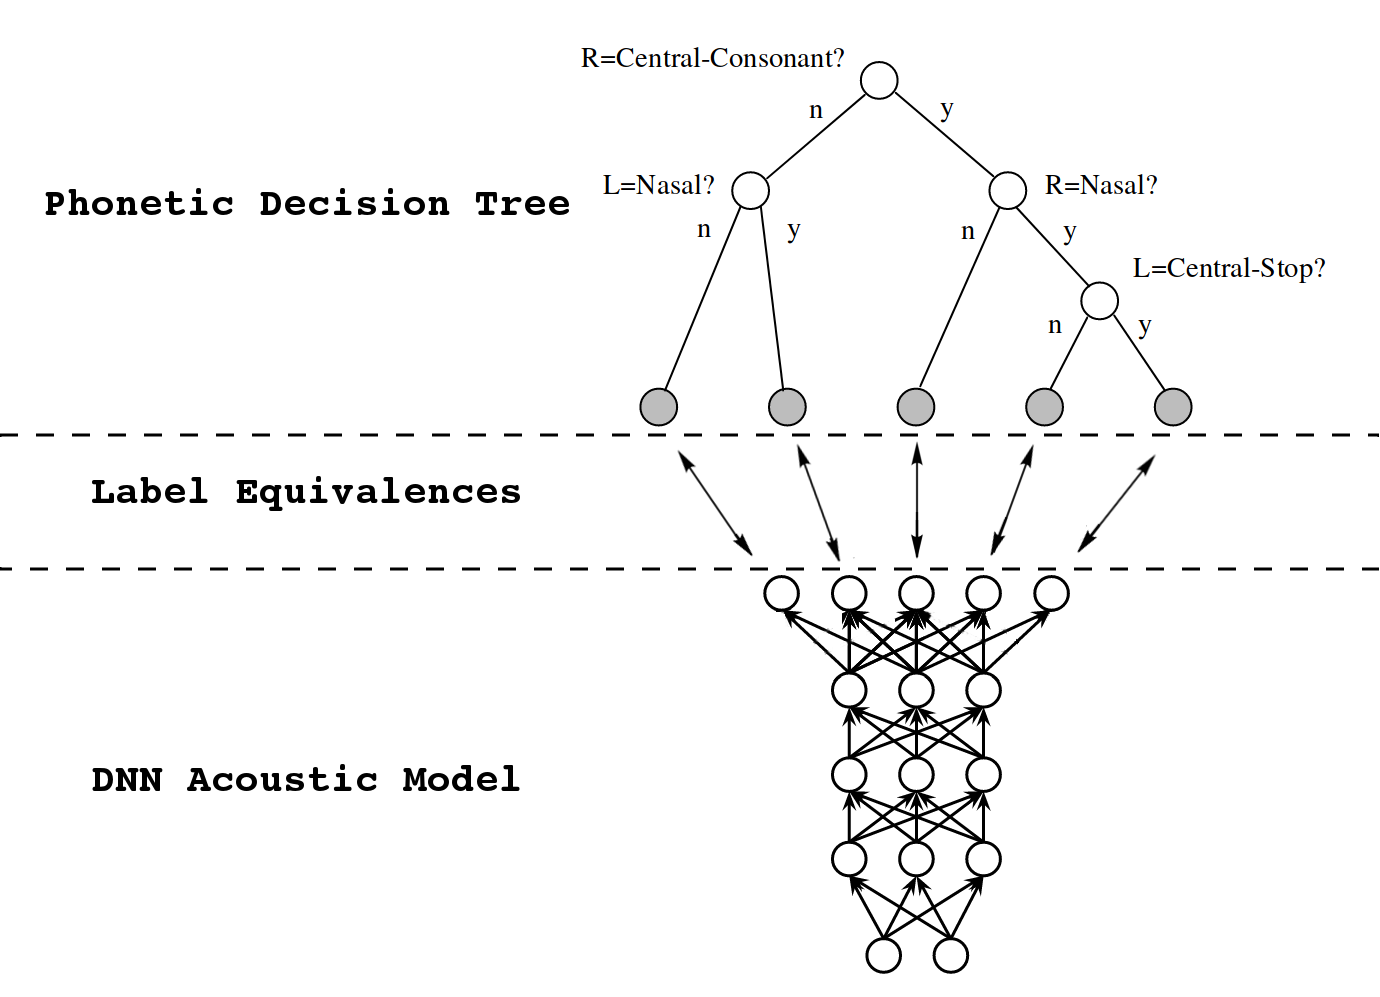
\includegraphics[width=\linewidth]{figs/tree-net.png}
          \caption{Label Correspondance of Decision Tree / DNN }
          \label{fig:mtl-dnn}
          \endminipage\hfill
        \end{figure}

        \vfill

        
        \begin{block}{\boxnumber Alignment}
          \begin{itemize}
          \item Feature Extraction
            \begin{itemize}
            \item 13 PLP features, 25ms Hamming windows, 10ms shift, 16 frame left-context \& 12 frame right-context, CMVN
            \end{itemize}
          \item GMM Alignment
            \begin{itemize}
            \item Monophones: 1,000 Gaussians, 25 iterations EM // Triphones: 2,000 leaves \& 5,000 Gaussians, 25 iterations EM
            \end{itemize}
          \end{itemize}
        \end{block}
  
        \vfill


                \begin{block}{\boxnumber Clustering}            
          \begin{itemize}
          \item k-means Clustering
            \begin{itemize}
            \item A set number of clusters is discovered via TensorFlow's standard k-means clustering.
            \end{itemize}
          \end{itemize}
        \end{block}

                
      } % end of parbox
    \end{column}

    %% Next column:
    %% ============================================================
    \begin{column}{0.3\textwidth}

      \parbox[t][\columnheight]{.9\textwidth}{
        
        \vspace{.4cm}

                
                \begin{block}{\boxnumber Mapping Triphone States $\rightarrow$ Clusters}          
          \begin{itemize}
            \item All training examples aligned to triphone state are mapped to most common k-means cluster.
          \end{itemize}
                \end{block}

                \vfill
                
        \begin{figure}[!htbp]
          \centering
          \minipage{\textwidth}
          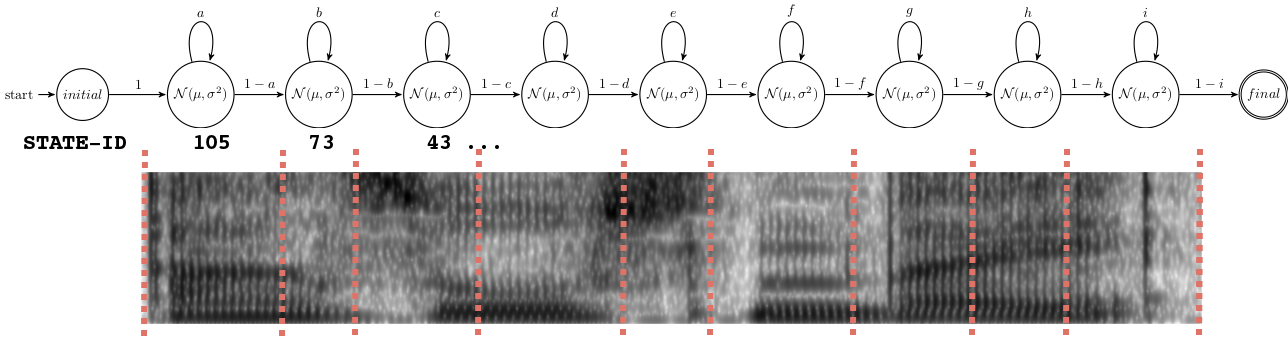
\includegraphics[width=\linewidth]{figs/aligned.png}
          \caption{GMM-aligned training examples}
          \endminipage\hfill
        \end{figure}

        \vfill

        \begin{figure}[!htbp]
          \centering
          \minipage{\textwidth}
          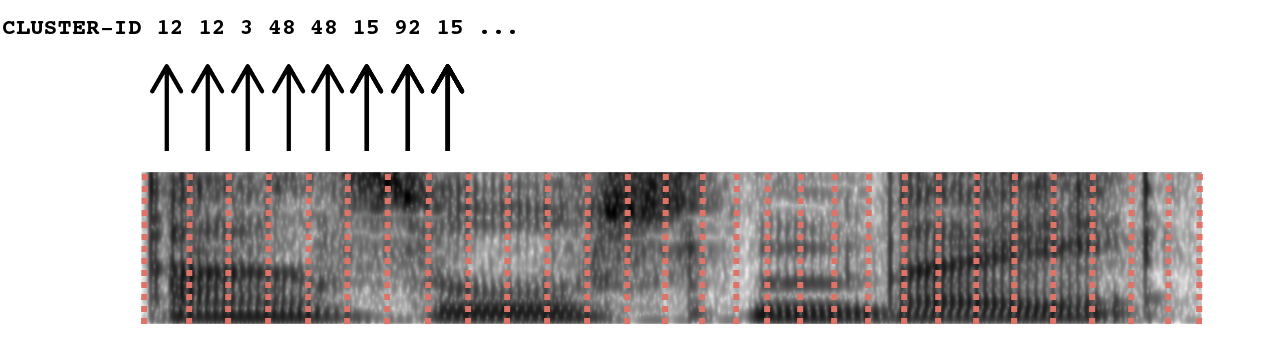
\includegraphics[width=\linewidth]{figs/clustered.png}
          \caption{k-means clustered training examples}
          \endminipage\hfill
        \end{figure}
        
        \vfill
        
        
        \begin{figure}[!htbp]
          \centering
          \minipage{\textwidth}
          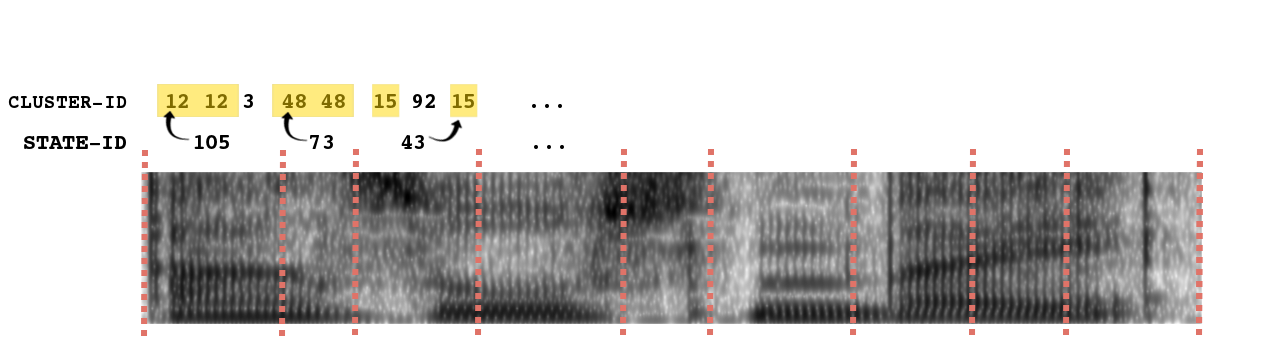
\includegraphics[width=\linewidth]{figs/mapped.png}
          \caption{GMM-aligned training examples}
          \endminipage\hfill
        \end{figure}

        \vfill


                
        \begin{block}{\boxnumber Cluster Contents}
          
          \begin{itemize}
          \item 672 leaves in Kaldi and 1024 clusters in TF
          \item 185 new labels after mapping
            \begin{itemize}
            \item 123 / 185 are interpretable
            \end{itemize}
          \item 84 / 185 contain only one phoneme
            \begin{itemize}
            \item 9 / 84 contained $>1$ triphone of phoneme
            \end{itemize}
          \item 101 / 184  contain mixed phonemes
            \begin{itemize}
            \item 39 / 101 only vowels or only consonants
            \end{itemize}
          \end{itemize}
          
        \end{block}

        \vfill
        
          \begin{table}[!htbp]
            \centering
            \caption{Discovered intelligible Phoneme Clusters}
            \label{tab:results}
            \begin{adjustbox}{width=.5\textwidth}
              \begin{tabular}{llrr}
                \toprule
                \multicolumn{2}{c}{Vowels} &  \multicolumn{2}{c}{ Consonants} \\
                \midrule
                a  j & a  u  &   k  r &     g n m \\
                a  o & a  ih  &    k p  &    s sh ch\\
                e  j & e  ih & r ng & t k s p \\
                e  y &o  u & d ch & m ng\\
                u  ih  y   & u  ih & t k & t k h\\
                i  e  y &o  ih & d z&t k s \\
                a  e  oe  j ih & j ih & l z  & t ch d\\
                a  ih  o  u  y &  &  n p & t k zh b  \\
                &&& t g b s sh z zh \\
                \bottomrule
              \end{tabular}
            \end{adjustbox}
          \end{table}


                  \vfill
        
        \begin{block}{\boxnumber Multi-Task DNN Training Set-up}          
          \begin{itemize}    
          \item DNN Acoustic model training
            \begin{itemize}
            \item Multi-Task Time-Delay Neural Network
            \item 5-epochs, 11 hidden layers, $ReLU$ activations
            \item $\alpha_{initial}=0.0015$ $\rightarrow$ $\alpha_{final}=0.00015$
            \item Each task has penultimate + ultimate output layer
            \end{itemize}
          \end{itemize}
        \end{block}

        \vfill

        \begin{figure}[!htbp]
          \centering
          \minipage{\textwidth}
          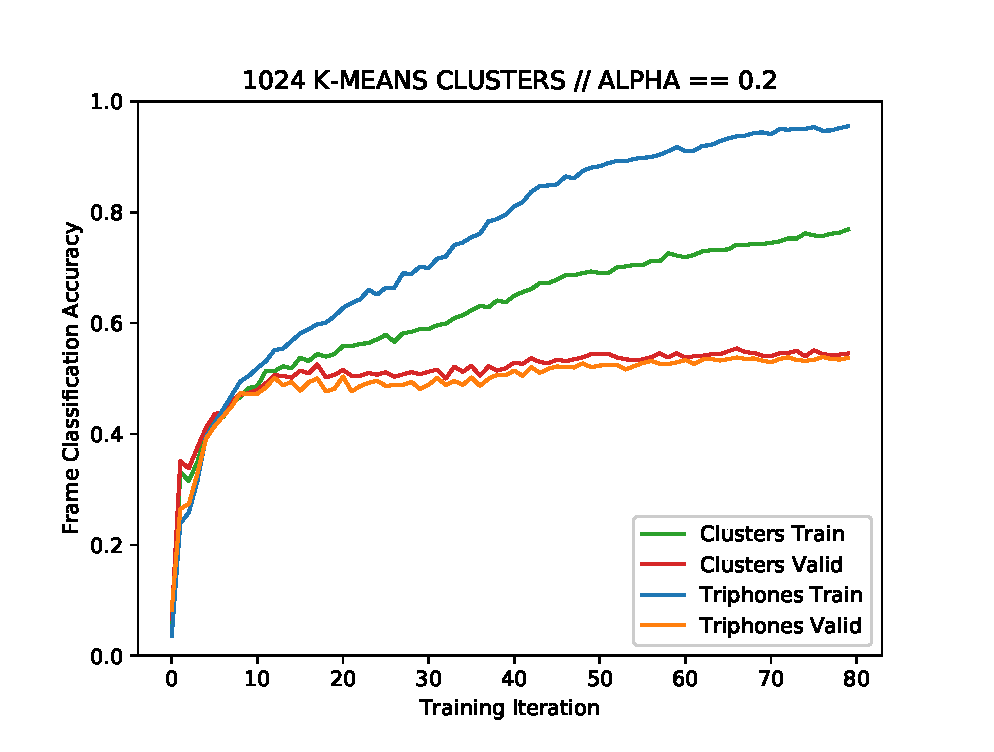
\includegraphics[width=\linewidth]{figs/1_point_2_1024.eps}
          \caption{Model Accuracy During Training (Simple Loss)}
          \endminipage\hfill
        \end{figure}

        

        
      } % end of parbox
    \end{column}

    
    %% Next column:
    %% ============================================================
    \begin{column}{0.3\textwidth}
      \parbox[t][\columnheight]{.9\textwidth}{
        \vspace{1cm}               % automatically nicely spaced out.

        
        \begin{block}{\boxnumber Testing Setup}
          \begin{itemize}
          \item k-folds cross-validation ($k==5$)
            \begin{itemize}
            \item 511 utterances for train
            \item 100 utterances for test
            \end{itemize}
            \item Decoded with 1-gram LM      
          \end{itemize}
        \end{block}

        \vfill
        
        \begin{block}{\boxnumber Results: Traditional Weighting Scheme}
          \begin{itemize}
          \item Loss = $((1-\alpha)*MAIN + \alpha*AUX)$
          \item WER better than Baseline in 4/9 experiments
          \end{itemize}
        \end{block}

        
        \vfill
        

                  
          \begin{table}[!htbp]
            \centering
            \caption{WER\% for Traditional Weighting Scheme}
            \begin{adjustbox}{width=\textwidth}
              \begin{tabular}{lccc}
                \toprule
                & $\alpha = 0.1 $ & $\alpha = 0.2 $ & $\alpha = 0.3 $\\
                \midrule
                Single Task Baseline  &  \multicolumn{3}{c}{$57.55$ \raisebox{.33\height}{\footnotesize{$\pm 1.82$}}}     \\
                
                \textbf{+ 256 clusters}  &  $57.93$ \raisebox{.33\height}{\footnotesize{$\pm 1.63$}}   &  $57.04$ \raisebox{.33\height}{\footnotesize{$\pm 1.58$}}     & 57.66 \raisebox{.33\height}{\footnotesize{$\pm 1.24$}} \\
                
                \textbf{+ 1024 clusters}   & $57.69$ \raisebox{.33\height}{\footnotesize{$\pm 3.78$}}    & \textbf{56.99} \raisebox{.33\height}{\footnotesize{$\pm 3.08$}}    & $57.60$ \raisebox{.33\height}{\footnotesize{$\pm 0.79$}}  \\
                
                \textbf{+ 4096 clusters}   &  $57.25$ \raisebox{.33\height}{\footnotesize{$\pm 2.87$}}  & $58.07$ \raisebox{.33\height}{\footnotesize{$\pm 1.35$}}   &   $57.45$ \raisebox{.33\height}{\footnotesize{$\pm 0.32$}}  \\
                \bottomrule
              \end{tabular}
            \end{adjustbox}
          \end{table}


          \vfill
          
        
        \begin{block}{\boxnumber Results: Simple Weighting Scheme}
          \begin{itemize}
          \item Loss = $(MAIN + \alpha*AUX$)
          \item WER better than Traditional Loss
          \item WER better than Baseline in 6/9 experiments
          \end{itemize}
        \end{block}        

        \vfill
        
        
        \begin{table}[!htbp]
          \centering
          \caption{WER\% for Simple Weighting Scheme}
          \begin{adjustbox}{width=\textwidth}
            \begin{tabular}{lccc}
              \toprule
              & $\alpha = 0.1 $ & $\alpha = 0.2 $ & $\alpha = 0.3 $\\
              \midrule
              Single Task Baseline  &  \multicolumn{3}{c}{$57.55$ \raisebox{.33\height}{\footnotesize{$\pm 1.82$}}}     \\
              
              \textbf{+ 256 clusters}  &  $57.33$ \raisebox{.33\height}{\footnotesize{$\pm 2.49$}}   &  $58.02$ \raisebox{.33\height}{\footnotesize{$\pm 2.09$}}     & $57.18$ \raisebox{.33\height}{\footnotesize{$\pm 0.56$}} \\
              
              \textbf{+ 1024 clusters}   & $ 57.74$ \raisebox{.33\height}{\footnotesize{$\pm 3.06$}}    & \textbf{56.88}  \raisebox{.33\height}{\footnotesize{$\pm 1.33$}}    & $57.13  $ \raisebox{.33\height}{\footnotesize{$\pm 1.55$}}  \\
              
              \textbf{+ 4096 clusters}   &  $57.56$ \raisebox{.33\height}{\footnotesize{$\pm 2.53$}}  & $57.49$ \raisebox{.33\height}{\footnotesize{$\pm  3.17$}}   &  $57.31$ \raisebox{.33\height}{\footnotesize{$\pm 1.31$}}  \\
              \bottomrule
            \end{tabular}
          \end{adjustbox}
        \end{table}
        
        \vfill


                \begin{block}{\boxnumber Discussion}
          \begin{itemize}
          \item Good auxiliary tasks exist (we just need to find them)
          \item Initial Results show small improvements, given good hyper-parameters
          \item Clustering in high-dimensional feature space isn't great
                  \begin{itemize}
                  \item Find better projections: LDA, source DNN activations (from well-resourced lang)
                  \end{itemize}
                \item Big net overfits to both tasks
                            \begin{itemize}
                            \item add more tasks
                            \item use smaller net
                            \end{itemize}
          \end{itemize}
        \end{block}        

        \vfill
        


        
        
        \begin{block}{\boxnumber Acknowledgements}
          \footnotesize{This material is based upon work supported by the National Science Foundation Graduate Research Fellowship under Grant No. (DGE-1746060). Any opinion, findings, and conclusions or recommendations expressed in this material are those of the authors(s) and do not necessarily reflect the views of the National Science Foundation.}
        \end{block}

        
        }%parbox
    \end{column}
    
  \end{columns}
\end{frame}

\end{document}
